\documentclass[resume]{subfiles}


\begin{document}
\section{Stocks \& Flows}
\subsection{Diagrammes de boucles causales}
\begin{center}
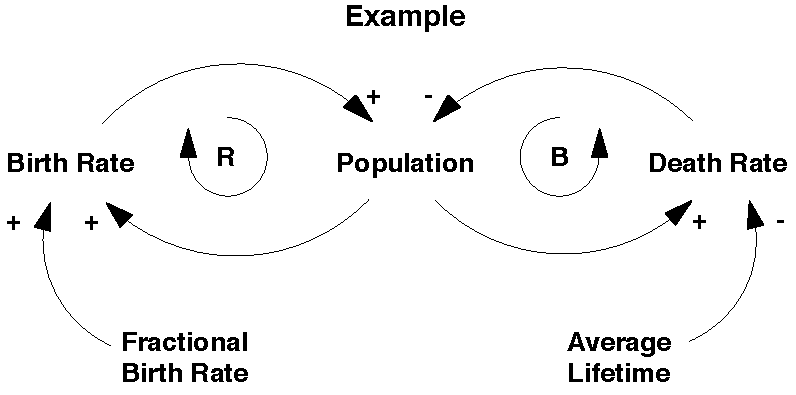
\includegraphics[scale=0.4,page=1]{img_0.pdf}\\
\includegraphics[scale=0.4,page=2]{img_0.pdf}\\
\includegraphics[scale=0.4,page=3]{img_0.pdf}
\end{center}
Mettre des noms plutôt que des phrases et éviter les négations inutiles
\subsubsection{Polarité de boucle}
Multiplication de toutes les polarités.
\subsection{Stocks}
État d'un système
$$\text{stock}(t)=\int_{t_0}^{t}\text{in}(s)-\text{out}(s)ds+\text{stock}(t_0)$$
\begin{itemize}
\item Caractérisation de l'état d'un système
\item Mémoire ou inertie
\item Génération de retard
\end{itemize}
\subsection{Flux (Flows)}
Les flux changent les stocks
$$\frac{d\text{stock}(t)}{dt}=\text{in}(t)-\text{out}(t)$$







\end{document}